\documentclass[11pt,fleqn]{article}
%\usepackage{CJK}
\usepackage{latexsym}
\usepackage{color}
\usepackage{graphicx, float}\usepackage{graphicx}
%\usepackage{algorithmicx}
\usepackage{algorithm}
\usepackage{algpseudocode}
%\usepackage[colorlinks]{hyperref}
\setlength{\oddsidemargin}{-0.0in}
\setlength{\evensidemargin}{-0.0in} \setlength{\textwidth}{6.0in}
\setlength{\textheight}{9.0in} \setlength{\topmargin}{-0.2in}

%\setlength{\leftmargin}{0.7in}
\usepackage{amssymb, graphicx, amsmath}  %  fancyheadings,
\usepackage{setspace}
\newcommand\qed{\qquad $\square$}
\newcommand{\nn}{\nonumber}

\def \[{\begin{equation}}
\def \]{\end{equation}}
\def\proof{{\bf Proof:\quad}}
\def \endzm {\quad $\Box$}
\def\dist{\hbox{dist}}


\newcommand{\R}{\mathbb{R}}
%\newtheorem{yinli}{����}[section]
\newcommand{\D}{\displaystyle}
\newcommand{\T}{\textstyle}
\newcommand{\SC}{\scriptstyle}
\newcommand{\FT}{\footnotesize}



%\newtheorem{theorem}{Theorem}[section]
%\renewcommand{\thetheorem}{\arabic{section}.\arabic{theorem}}
\newtheorem{definition}{Definition}
\renewcommand{\thedefinition}{\arabic{section}.\arabic{definition}}
\newtheorem{lemma}{Lemma}[section]
\renewcommand{\thelemma}{\arabic{section}.\arabic{lemma}}
\newtheorem{remark}{Remark}
\renewcommand{\theremark}{\arabic{section}.\arabic{remark}}
\newtheorem{proposition}{Proposition}[section]
\renewcommand{\theproposition}{\arabic{section}.\arabic{proposition}}
\newtheorem{corollary}{Corollary }[section]
\renewcommand{\thecorollary}{\arabic{section}.\arabic{corollary}}
\renewcommand{\theequation}{\arabic{section}.\arabic{equation}}
\renewcommand{\baselinestretch}{1.35}
\newtheorem{exam}{Example}[section]
\renewcommand{\theexam}{\arabic{section}.\arabic{exam}}
\newtheorem{theo}{Theorem}[section]
\renewcommand{\thetheo}{\arabic{section}.\arabic{theo}}
\begin{document}
%\begin{CJK*}{GBK}{song}

\begin{center}

{\LARGE \bf  Natural Language Processing Assignment 1}\\

\vskip 5pt
 {Huihuang Zheng, huihuang@utexas.edu }\\
\vskip 5pt
{\small hz4674 Spring 2016 }

\end{center}
\begin{spacing}{1}

\section{Using Code}
To run me code, put your data folders of \emph{atis, wsj, brown} in the folder \textbf{PartOfSpeechTaggedData/} then you just need to run \textbf{run.sh} (using \emph{bash} \textbf{run.sh} in Linux terminal). It will show trace file analogous to the BigramModel trace file on course page in the terminal. You can also run \textbf{run\_and\_output\_to\_file.sh} (using \emph{bash} \textbf{run\_and\_output\_to\_file.sh} in Linux terminal). That will show trace file in the terminal and generate a file \textbf{./traceFile/traceFile.txt}. You can see trace file for all three models in the \textbf{traceFile.txt}.

\section{How did I implement}
\subsection{BackwardBigramModel}
For \textbf{BackwardBigramModel}, the easiest way to implement it is to reverse the sentences when train and predict, and then do same thing as \textbf{BigramModel}. So I reverse the input sentences and then call \textbf{BigramModel}'s method \emph{trainSentence}, \emph{sentenceLogProb}, \emph{sentenceLogProb2}, \emph{sentenceTokenProbs}.
\subsection{BidirectionalBigramModel}
To implement \textbf{BidirectionBigramModel}, I train two model \textbf{BigramModel} and \textbf{BackwardBigramModel} for sentences. Then combine their results. In this model, we are trying to get prediction of token T from (left, T, right) by combine of unigram (T), forward bigram model (left, T) and backward bigram model (T, right). I set same weight for bigram and backward bigram. That is, my prediction for token T is

$$p(T) = \frac{1}{2}p_{forward} + \frac{1}{2}p_{backward}$$.

Notice that the
$$p_{forward} = \frac{1}{2}p(T) + \frac{1}{2}p(T|left)$$
$$p_{backward} = \frac{1}{2}p(T) + \frac{1}{2}p(T|right)$$
So my prediction for token T is
$$p(T) = \frac{1}{2}p(T) + \frac{1}{4}p(T|left) + \frac{1}{2}p(T|right)$$

In addition, the prediction for whole sentence is that we multiple prediction of all tokens together.
\section{Experiment}
I used 90\% data from atis, wsj and brown for training and remaining 10\% for testing. My result is:\\
\begin{center}
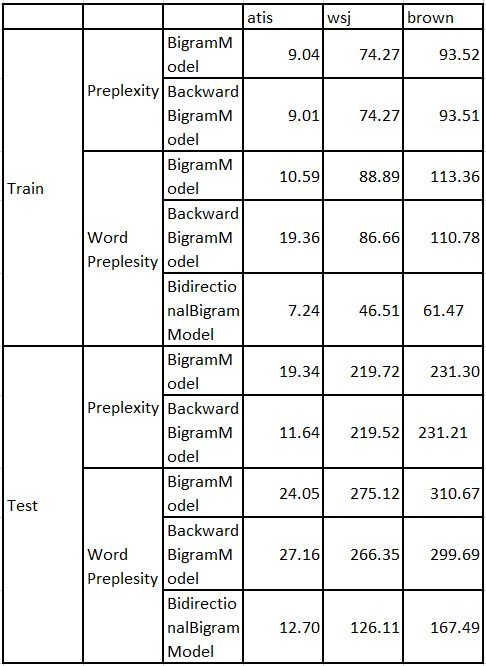
\includegraphics[width=0.75\linewidth]{table.JPG}
\end{center}
\section{Result Analysis}
From the table, we can see if we use \textbf{BigramModel} and \textbf{BackwardBigramModel} each, the preplexity doesn't change a lot. But if we combine them together, the word preplexity of bidirectiondecreases a lot. The reason should be the backward bigram model does something similar to forward bigram model. So the result is similar. But the \textbf{BidirectionBigramModel} have both information from forward and backward. It can get lower word preplexity.

\end{spacing}

%\end{CJK*}
\end{document}
